\documentclass{article}
\usepackage{graphicx} % Required for inserting images
\usepackage{amsmath}
\usepackage{amssymb} % used for math symbols
\usepackage{mathtools}
\usepackage{enumitem}
\usepackage{wasysym}
\usepackage{float}


\title{Computer Grafik Blatt 6}
\date{June 2023}

\begin{document}

\maketitle

\section*{Aufgabe 1.}
\subsection*{a)}
\begin{table}[H]
    \begin{tabular}{l|l|l|l|}
        \cline{2-4}
                                                                                                                                                                          & attribute       & uniform         & varying         \\ \hline
        \multicolumn{1}{|l|}{Wert kann im Vertex Shader gelesen werden}                                                                                                   & \hfil\checkmark & \hfil\checkmark & \hfil\checkmark \\ \hline
        \multicolumn{1}{|l|}{\begin{tabular}[c]{@{}l@{}}Wert kann Vertex Shader geschrieben und ge-\\ ändert werden\end{tabular}}                                         &                 &                 & \hfil\checkmark \\ \hline
        \multicolumn{1}{|l|}{\begin{tabular}[c]{@{}l@{}}Kann im Vertex Shader innerhalb einer Funkti-\\ on definiert werden\end{tabular}}                                 &                 &                 &                 \\ \hline
        \multicolumn{1}{|l|}{\begin{tabular}[c]{@{}l@{}}Hat im Vertex Shader grundsätzlich für jeden\\ Vertex den gleichen Wert\end{tabular}}                             &                 & \hfil\checkmark &                 \\ \hline
        \multicolumn{1}{|l|}{Wert kann im Fragment Shader gelesen werden}                                                                                                 &                 & \hfil\checkmark & \hfil\checkmark \\ \hline
        \multicolumn{1}{|l|}{\begin{tabular}[c]{@{}l@{}}Wert kann im Fragment Shader geschrieben\\ und geändert werden\end{tabular}}                                      &                 &                 &                 \\ \hline
        \multicolumn{1}{|l|}{\begin{tabular}[c]{@{}l@{}}Kann im Fragment Shader innerhalb einer\\ Funktion definiert werden\end{tabular}}                                 &                 &                 &                 \\ \hline
        \multicolumn{1}{|l|}{\begin{tabular}[c]{@{}l@{}}Hat im Fragment Shader grundsätzlich für je-\\ des Fragment des selben Dreiecks den gleichen\\ Wert\end{tabular}} &                 & \hfil\checkmark &                 \\ \hline
        \multicolumn{1}{|l|}{\begin{tabular}[c]{@{}l@{}}Wert kann im Hauptprogramm geschrieben\\ und geändert werden\end{tabular}}                                        & \hfil\checkmark & \hfil\checkmark &                 \\ \hline
    \end{tabular}
\end{table}

\subsection*{b)}
Die finale Position eines Vertex muss im \underline{Vertex} Shader in die eingebaute Variable \underline{gl\_Position} geschrieben werden. \\
Die finale Farbe eines Fragments muss im \underline{Fragment} Shader in die eingebaute Variable \underline{gl\_FragColor} geschrieben werden.

\subsection*{c)}
% list that can have different label for each item
\begin{itemize}[label=$\square$]
    \item ModelView-Transformation
    \item Projektion
    \item[\CheckedBox] Rasterisierung
    \item z-Buffer-Test
\end{itemize}
% Macht man ModelView-Transformation und Projektion nicht selbst manuell im Vertex Shader?
% Findet z-Buffer-Test im Fragment Shader oder davor statt?

\subsection*{d)}
$4096 \cdot 2304 = 9437184$ Pixel. Der Fragment Shader wird somit mindestens $9437184$ mal aufgerufen.
Gibt es mehrere überlappende Objekte, so wird der Fragment Shader öfter aufgerufen. (??)


\subsection*{e)}
\begin{enumerate}
    \item vec4 v = vec4(1.0, 2.0, 3.0, 4.0);
    \item float x = 8;
          \begin{itemize}
              \item 8 ist ein integer, 8 als float wäre 8.0
          \end{itemize}
    \item vec3 v1 = v.xxx;
    \item vec3 v2 = v.xyzw;
          \begin{itemize}
              \item vec3 bekommt vec4 zugewiesen
          \end{itemize}
    \item float f = v[1];
    \item v[0] = f;
    \item vec3 w = vec3(5.0, 6.0, 7.0);
    \item mat2 m = mat2(2.0, 3.0, 1.0, 0.0, 0.1);
          \begin{itemize}
              \item mat2 bekommt 5 Werte übergeben, obwohl nur 4 benötigt werden
          \end{itemize}
    \item vec3 v3 = v.gb;
          \begin{itemize}
              \item vec3 wird vec2 zugewiesen
          \end{itemize}
    \item vec3 v4 = v.abc;
          \begin{itemize}
              \item abc sind keine gültigen Werte
          \end{itemize}
    \item vec3 d = dot(w, v1);
          \begin{itemize}
              \item dot() gibt float zurück und nicht vec3
          \end{itemize}
    \item vec3 e = dot(v.ab, w.xy);
          \begin{itemize}
              \item dot() gibt float zurück und nicht vec3
          \end{itemize}
    \item vec3 r = cross(w, v);
          \begin{itemize}
              \item cross() von vec3 und vec4 nicht möglich
          \end{itemize}
    \item v[1] = x;
\end{enumerate}

\subsection*{f)}
Der Fragment Shader wird für jedes Pixel ausgeführt, aber nur die Pixel, welche im Dreieck liegen, werden gezeichnet.
Das Dreieck nimmt bei den gegebenen Koordinaten ca. 1/4 des Bildschirms ein, also werden ca. 25\% der Pixel nicht mehr schwarz sein. (??)\\~\\

Das Dreieck wird bei der Rasterisierung geclipt. Vermutlich auf (0,0,0,1),(1,-1,0.25,1),(-1,-1,0.0625,1). Danach wird für jedes Fragment des Dreiecks die Farbe auf (0,0,1,1) also Blau mit voller Opazität gesetzt. Nach dem Fragmentshader wird dann für jeden Pixel der Verdeckungstest gemacht, und da das Dreieck vollständig vor dem maximalwert 1 liegt werden alle pixel die fragmente des Dreieck enthalten Blau bemalt. Alle übrigen Pixel werden Schwarz bemalt, da hier die im Color-Buffer gesetzte Frabe genutzt wird. Final erhalten wir ein blaues Dreieck von der mitte zu beiden unteren Ecken mit einem schwarzen Hintergrund. Somit sind ziemlich genau 25\%  der Pixel nicht mehr Schwarz.

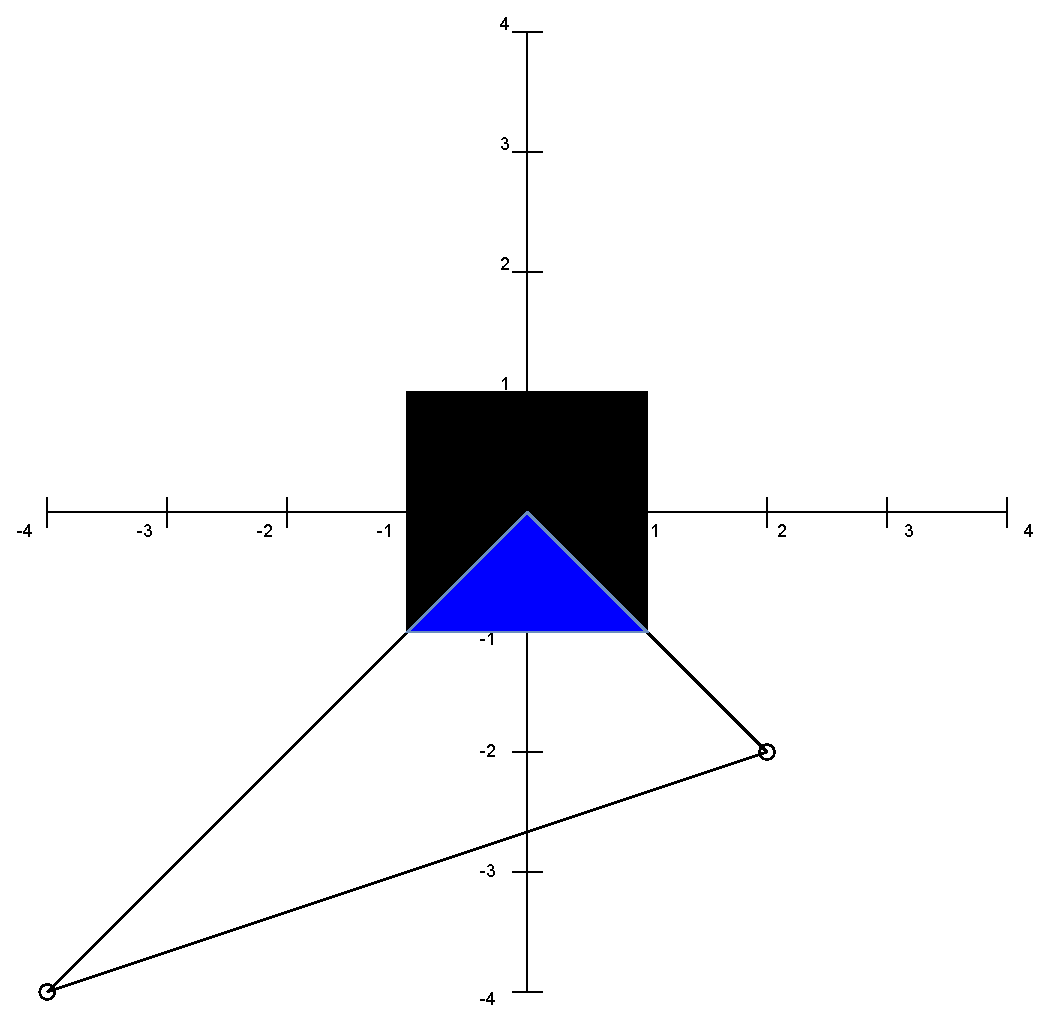
\includegraphics[width=\textwidth, keepaspectratio]{CG6.1.f.drawio.pdf}

\end{document}